% !TEX program = lualatex
%% FullCourse_10Lecs -- Lecture 1, Topic 1.2: AI as a Research Collaborator
%% New for the re-pitched opening: AI *doing* frontier economic research.
%% Case A (DeepRamsey) condensed from Lec10_T8_Case6_DeepRamsey.tex.
%% Case B (GRAM) reproduced as inline TikZ from the GRAM slides (slides_v3).
%% Research-map + live WIP frames migrated verbatim from the old Lec02_T2.

%% Shared preamble for the FullCourse_10Lecs topic decks.
%%
%% Each topic .tex \input's this file, then defines its own \title, \date
%% override (if any), \graphicspath, and \begin{document}.
%%
%% Reconstructed verbatim from the inlined copy preserved in
%% Lec10_Case_Studies/Lec10_T8_Case6_DeepRamsey.tex (lines 23-190), which is
%% explicitly annotated there as "from ../shared_preamble.tex, copied verbatim".
%% Base preamble matches MiniCourse_8hr/Slides/shared_preamble.tex; this version
%% additionally provides \sectiondivider, the conceptbox/cautionbox/examplebox/
%% takeawaybox tcolorboxes, and \compacttables used across the split decks.

\documentclass[10pt,english,aspectratio=169]{beamer}

\usepackage{ae,aecompl}
\usepackage[T1]{fontenc}
\usepackage{textcomp}
\usepackage[utf8]{inputenc}
\usepackage{babel}
\usepackage{datetime2}

\setcounter{secnumdepth}{3}
\setcounter{tocdepth}{3}

\usepackage{amsmath, amssymb, amsthm, graphicx}
\usepackage{booktabs, multirow}
\usepackage{tikz}
\usepackage{pgfplots}
\pgfplotsset{compat=1.16}
\usepackage[most]{tcolorbox}
\tcbuselibrary{skins, breakable, theorems}
\usepackage{listings}
\usepackage{xcolor}

\lstset{
  basicstyle=\ttfamily\small,
  keywordstyle=\color{blue!80!black}\bfseries,
  commentstyle=\color{green!50!black}\itshape,
  stringstyle=\color{orange!80!black},
  backgroundcolor=\color{gray!8},
  frame=single,
  rulecolor=\color{gray!40},
  breaklines=true,
  showstringspaces=false,
  numbers=none,
}

\lstdefinestyle{pythonstyle}{
    language=Python,
    basicstyle=\ttfamily\footnotesize,
    keywordstyle=\color{blue!80!black}\bfseries,
    commentstyle=\color{green!50!black}\itshape,
    stringstyle=\color{orange!80!black},
    frame=single,
    breaklines=true,
    showstringspaces=false,
    numbers=left,
    numbersep=5pt,
    numberstyle=\tiny\color{gray},
    backgroundcolor=\color{gray!8},
    rulecolor=\color{gray!40}
}

\ifx\hypersetup\undefined
  \AtBeginDocument{%
    \hypersetup{bookmarks=false,breaklinks=true,pdfborder={0 0 0},colorlinks=true,
      linkcolor=DarkText,urlcolor=RedTitle}%
  }
\else
  \hypersetup{bookmarks=false,breaklinks=true,pdfborder={0 0 0},colorlinks=true,
    linkcolor=DarkText,urlcolor=RedTitle}%
\fi

\makeatletter
\newcommand\makebeamertitle{%
  \begin{frame}[plain]
    \vspace*{1.0cm}
    \centering
    {\usebeamerfont{title}\usebeamercolor[fg]{title}\inserttitle\par}
    \vspace{1.0cm}
    {\usebeamerfont{author}\usebeamercolor[fg]{author}\insertauthor\par}
    \vspace{0.2cm}
    {\usebeamerfont{date}\usebeamercolor[fg]{date}\insertdate\par}
  \end{frame}}%
\AtBeginDocument{%
  \let\origtableofcontents=\tableofcontents
  \def\tableofcontents{\@ifnextchar[{\origtableofcontents}{\gobbletableofcontents}}
  \def\gobbletableofcontents#1{\origtableofcontents}%
}

\usetheme{metropolis}
\usefonttheme{professionalfonts}

\definecolor{LightGray}{RGB}{230,230,230}
\definecolor{RedTitle}{RGB}{0,0,200}
\definecolor{VeryLightGray}{RGB}{245,245,245}
\definecolor{DarkText}{RGB}{0,0,0}

\setbeamercolor{background canvas}{bg=white}
\setbeamercolor{title}{fg=RedTitle}
\setbeamercolor{author}{fg=DarkText}
\setbeamercolor{date}{fg=DarkText}
\setbeamercolor{frametitle}{bg=VeryLightGray,fg=DarkText}
\setbeamercolor{normal text}{fg=DarkText}
\setbeamerfont{title}{size=\large}

\setbeamersize{text margin left=5mm, text margin right=5mm}
\addtobeamertemplate{frametitle}{}{\vspace{-0.5em}}
\newcommand{\reducevspace}{\vspace{-0.5cm}}

% Shared section divider and box styles for split topic decks.
\newcommand{\sectiondivider}[2]{%
\begin{frame}[plain,noframenumbering]
\begin{center}
\vfill
{\Large\textbf{#1}\par}
\vspace{0.35cm}
{\normalsize #2\par}
\vfill
\end{center}
\end{frame}
}

\newtcolorbox{conceptbox}[1][]{
  colback=blue!3,
  colframe=RedTitle!55,
  boxrule=0.35mm,
  arc=1mm,
  left=2mm,
  right=2mm,
  top=1mm,
  bottom=1mm,
  #1
}
\newtcolorbox{cautionbox}[1][]{
  colback=red!3,
  colframe=red!50!black,
  boxrule=0.35mm,
  arc=1mm,
  left=2mm,
  right=2mm,
  top=1mm,
  bottom=1mm,
  #1
}
\newtcolorbox{examplebox}[1][]{
  colback=green!3,
  colframe=green!45!black,
  boxrule=0.35mm,
  arc=1mm,
  left=2mm,
  right=2mm,
  top=1mm,
  bottom=1mm,
  #1
}
\newtcolorbox{takeawaybox}[1][]{
  colback=VeryLightGray,
  colframe=RedTitle!55,
  boxrule=0.35mm,
  arc=1mm,
  left=2mm,
  right=2mm,
  top=1mm,
  bottom=1mm,
  #1
}
\newcommand{\compacttables}{\renewcommand{\arraystretch}{1.15}}

\setbeamertemplate{navigation symbols}{}
\setbeamertemplate{footline}{%
  \hfill%
  \usebeamercolor[fg]{page number in head/foot}%
  \usebeamerfont{page number in head/foot}%
  \insertframenumber\,/\,\inserttotalframenumber\kern1em\vskip2pt%
}

\makeatother

\author{Zhigang Feng}
% "date with time": compile timestamp so each build is identifiable.
\date{\today\ \DTMcurrenttime}


% --- CJK: real characters under Lua/XeLaTeX; English fallback under pdfLaTeX ---
\usepackage{iftex}
\ifluatex
  \usepackage{luatexja-fontspec}
  \setmainfont{Latin Modern Roman}%
  \setsansfont{Latin Modern Sans}%
  \setmonofont{Latin Modern Mono}%
  \setmainjfont{FandolSong-Regular.otf}[BoldFont=FandolHei-Regular.otf]%
  \newcommand{\zhterm}[2]{#1}%
\else\ifxetex
  \usepackage{fontspec}
  \setmainfont{Latin Modern Roman}%
  \setsansfont{Latin Modern Sans}%
  \setmonofont{Latin Modern Mono}%
  \usepackage{xeCJK}
  \setCJKmainfont{FandolSong-Regular.otf}[BoldFont=FandolHei-Regular.otf]%
  \newcommand{\zhterm}[2]{#1}%
\else
  \newcommand{\zhterm}[2]{#2}% pdflatex: English fallback
\fi\fi
\newcommand{\bookAIforEcon}{\zhterm{苗建军、冯志钢：《面向经济学人的人工智能》，高等教育出版社，2027}{Miao \& Feng, \emph{Artificial Intelligence for Economists}, Higher Education Press, 2027}}

\graphicspath{{./figures/}{./pic/}{../../MiniCourse_8hr/Slides/Module1_ML_Foundations/pic/}{../}}

\usetikzlibrary{positioning,arrows.meta,shapes,calc,fit,backgrounds}

% Suppress the redundant auto-generated metropolis section page; the
% \sectiondivider frames below are the dividers we keep.
\metroset{sectionpage=none}
%% Lec01 shared MAP slide: "one map, three acts" recurring diagram.
%% Input this file AFTER ../shared_preamble.tex (needs RedTitle, VeryLightGray,
%% DarkText) and AFTER \usetikzlibrary{positioning,arrows.meta,shapes,calc}.
%% Call \LecOneMap{k} inside a frame, where k in {1,2,3} highlights the current
%% act ("you are here") and k = 0 renders the closing reprise with all three
%% acts checked green (used by T3's closing frame).
%% Filename deliberately does NOT match the build glob Lec*_T*.tex, so the build
%% script never tries to compile it standalone.
%%
%% The three acts are the lecture's story: FRAME -> PROOF -> PRACTICE, i.e.
%% AI framed as an economic object (cognitive capital), live proof that AI
%% already does frontier research (DeepRamsey, GRAM, measurement), and how
%% this course turns that into the student's own practice.

\newcommand{\LecOneMap}[1]{%
% Precompute per-box style selectors; TikZ option lists are comma-split before
% TeX conditionals run, so \ifnum must not sit inside a [...] options list.
\ifnum#1=0
  \tikzset{lmapa/.style={lmapdone}, lmapb/.style={lmapdone},
           lmapc/.style={lmapdone}}%
\else
  \tikzset{lmapa/.style={}, lmapb/.style={}, lmapc/.style={}}%
  \ifnum#1=1 \tikzset{lmapa/.style={lmapcur}}\fi
  \ifnum#1=2 \tikzset{lmapb/.style={lmapcur}}\fi
  \ifnum#1=3 \tikzset{lmapc/.style={lmapcur}}\fi
\fi
\begin{center}
\begin{tikzpicture}[
    act/.style={rectangle, rounded corners, draw=black!60, fill=VeryLightGray,
        minimum width=3.4cm, minimum height=1.0cm, text width=3.25cm,
        align=center, font=\small, text=DarkText},
    lmapcur/.style={draw=RedTitle, very thick, fill=orange!20},
    lmapdone/.style={draw=green!45!black, thick, fill=green!10},
    q/.style={font=\tiny\itshape, text width=3.4cm, align=center, text=black!70},
    barlab/.style={font=\tiny\bfseries, text=black!65},
    sat/.style={rectangle, rounded corners, draw=black!45, dashed, fill=white,
        text width=4.6cm, align=center, font=\tiny, text=black!70,
        minimum height=0.5cm},
    arr/.style={-{Stealth[length=2.4mm]}, thick, gray!60}
]
    % --- three act boxes ---
    \node[act, lmapa] (a1) at (0,0)
        {\textbf{1.1\ \ FRAME}\\[1pt] \tiny cognitive capital $\cdot$ growth};
    \node[act, lmapb] (a2) at (4.5,0)
        {\textbf{1.2\ \ PROOF}\\[1pt] \tiny DeepRamsey $\cdot$ GRAM $\cdot$ meas.};
    \node[act, lmapc] (a3) at (9.0,0)
        {\textbf{1.3\ \ PRACTICE}\\[1pt] \tiny roadmap $\cdot$ tooling $\cdot$ capstone};
    \draw[arr] (a1) -- (a2);
    \draw[arr] (a2) -- (a3);
    % --- the student question each act answers ---
    \node[q] at (0,-0.98)   {what kind of economic\\ object is AI?};
    \node[q] at (4.5,-0.98) {can AI actually do\\ frontier research?};
    \node[q] at (9.0,-0.98) {how does this course\\ make it mine?};
    % --- "you are here" marker above the current act ---
    \ifnum#1=1 \node[font=\scriptsize\bfseries, text=RedTitle] at (0,1.02)
        {you are here\ $\blacktriangledown$};\fi
    \ifnum#1=2 \node[font=\scriptsize\bfseries, text=RedTitle] at (4.5,1.02)
        {you are here\ $\blacktriangledown$};\fi
    \ifnum#1=3 \node[font=\scriptsize\bfseries, text=RedTitle] at (9.0,1.02)
        {you are here\ $\blacktriangledown$};\fi
    \ifnum#1=0 \node[font=\scriptsize\bfseries, text=green!45!black] at (4.5,1.02)
        {all three acts complete};\fi
    % --- bottom band: each act's memorable tagline (the lecture's spine) ---
    \fill[blue!10]   (-1.6,-1.78) rectangle (1.6,-1.45);
    \fill[green!12]  (2.9,-1.78)  rectangle (6.1,-1.45);
    \fill[orange!16] (7.4,-1.78)  rectangle (10.6,-1.45);
    \node[barlab] at (0,-1.615)   {PRICE OF COGNITION $\downarrow$};
    \node[barlab] at (4.5,-1.615) {CONTEXT, NOT CAPABILITY};
    \node[barlab] at (9.0,-1.615) {REPLICATION-FIRST};
    % --- dashed satellites: where this lecture sits in the course flow ---
    \node[sat] at (0,-2.45)
        {\textit{front door:} no prerequisites --- bring a research question and skepticism};
    \node[sat] at (9.0,-2.45)
        {\textit{downstream:} Lec02 opens the toolbox --- the predictive and generative stacks};
\end{tikzpicture}
\end{center}
}


\title[AI for Econ Research]{AI for Economic Research: Dynamic Models, Language, and Agents\\
Lecture 1.2: AI as a Research Collaborator}

\begin{document}

\makebeamertitle

%=============================================================================
\begin{frame}{Lecture 1 in One Map}
\textbf{One lecture, three decks, one claim: AI is new \emph{cognitive capital} --- cheap, fast, non-rival --- and this course trains you to deploy it on real research.}

\LecOneMap{2}

\vspace{0.05cm}
\footnotesize\textit{\textbf{Act 1.2 (here)} shows the claim in action: DeepRamsey co-develops a dynamic model, GRAM shows \emph{context --- not capability ---} is the bottleneck, the AI-for-research map places the tools (with causation as the standing guardrail), and a live measurement project asks what AI can actually \emph{finish}.}
\end{frame}

%=============================================================================
\section{Case A --- DeepRamsey}

\sectiondivider{Case A --- DeepRamsey}{AI as co-developer of a dynamic model --- and where human judgment stayed load-bearing}

\begin{frame}{AI Compresses the Theory$\to$Code Loop}
\textbf{Case study (full version: Lec.\ 10 T8): AI-assisted extension of the Feng, Han \& Zhu (2026) deep Ramsey solver from a representative-agent to a \emph{heterogeneous-agent} model --- a new paper, Chien, Feng \& Wen (in progress).}
\medskip
\begin{itemize}
    \item The theory--code--debug loop compressed \textbf{from months to days}: drafting, refactoring, auditing, and diagnostics stop being bottlenecks.
    \item Documentation became \emph{executable}: the TeX spec, audit notes, and code evolve in lockstep.
    \item \textbf{Where judgment stayed human:} the AI could not decide what was economically \emph{interesting}. It \emph{could} sometimes flag a mistimed equation or a non-credible number --- but confirming that stayed the economist's job.
\end{itemize}
\medskip
\begin{takeawaybox}\small
The AI supplies \textbf{throughput}; the economist supplies \textbf{judgment} --- the central lesson of the case.
\end{takeawaybox}
{\scriptsize Based on Feng, Han \& Zhu (2026), \emph{Ramsey Taxation, Public Debt Sustainability, and Asset Pricing in Incomplete Markets}; HA extension: Chien, Feng \& Wen (in progress).}
\end{frame}

\begin{frame}{Start From a Validated Seed --- Audit Before Extending}
\textbf{The conversation did not start with ``build me an HA model.'' It started with comprehension and audit tasks on the seed (the RA deep Ramsey solver):}
\smallskip
\begin{enumerate}\small
    \item \emph{Restate} the model and the algorithm; list every equation and where it is implemented.
    \item \emph{Audit} the code against the TeX: report every mismatch (scoring, bounds, sampling, penalties); classify each as a \textbf{correctness risk} or a \textbf{documentation gap}.
    \item \emph{Refine} to a consistent document+code pair --- add no new economics yet.
\end{enumerate}
\smallskip
\begin{conceptbox}\small
\textbf{Why audit first?} Extending an inconsistent seed propagates the inconsistency into every later version. The audit is the cheapest insurance in the whole project.
\end{conceptbox}
\end{frame}

\begin{frame}{Extend on Paper, Prototype with AI, Let Failures Teach}
\textbf{Milestone ladder:} refined RA $\to$ stripped-down HA model (\emph{TeX first}) $\to$ AI-built code (\texttt{v1}) $\to$ full model (\texttt{v2}), where \emph{debugging becomes architecture}.
\smallskip
\compacttables
\begin{center}\footnotesize
\renewcommand{\arraystretch}{1.05}
\begin{tabular}{p{6.6cm}cc}
\toprule
\textbf{Contribution} & \textbf{AI} & \textbf{Economist} \\
\midrule
Drafting/reorganizing LaTeX; vectorized PyTorch & \checkmark & \\
Proposing penalty \& boundary-learning patterns & \checkmark & \\
Summarizing diagnostics \& code/document mismatches & \checkmark & \\
Checking economic correctness of formulations & & \checkmark \\
Deciding which simplifications are acceptable & & \checkmark \\
Catching conceptual bugs (timing, transition direction) & & \checkmark \\
Setting validation benchmarks; accepting results & & \checkmark \\
\bottomrule
\end{tabular}
\end{center}
\end{frame}

\begin{frame}{Three Discoveries the Failures Forced}
\textbf{Hitting the \emph{same} failure, then asking \emph{why}, imported three tools economists rarely reach for:}
\smallskip
\begin{enumerate}\small
    \item \textbf{$\alpha$-shapes} (Edelsbrunner--M\"ucke 1994) to represent the \emph{generically non-convex} feasible set from sampled points --- surfaced when the boundary learner kept misclassifying near-kink states.
    \item \textbf{Viability kernel} (Aubin 1991) \emph{precedes} admissibility: the same monotone-set-operator structure as APS self-generation (Abreu--Pearce--Stacchetti 1990; Phelan--Stacchetti 2001; Feng 2015).
    \item A \textbf{Lyapunov-type penalty} for saddle-path selection under the $\beta R = 1$ unit root --- flat along the unit-root direction, punishing only the movement that signals divergence.
\end{enumerate}
\smallskip
\begin{examplebox}\small
\textbf{Pattern:} an ad hoc fix fails $\to$ AI-generated diagnostics isolate \emph{why} $\to$ the economist recognizes the deeper structure $\to$ joint design of the right tool. Cross-literature imports got \emph{cheap}.
\end{examplebox}
\end{frame}

\begin{frame}{Result: A Bistable Long Run}
\begin{columns}[T]
\begin{column}{0.52\textwidth}
\small
\textbf{Heterogeneity creates \emph{two} long-run outcomes:} full self-insurance (FSI), or \textbf{immiseration} (assets pile up, consumption collapses).
\smallskip
\begin{itemize}
    \item Which one is reached depends on \textbf{where the economy starts}.
    \item CRRA: only $\approx 13\%$ of initial conditions (a thin low-asset sliver) converge to FSI.
    \item Basin boundaries are thin and perturbation-sensitive --- mapped with the $\alpha$-shape machinery.
\end{itemize}
\smallskip
\begin{conceptbox}\small
\textbf{Long-run outcomes are history-dependent}: policy alone does not decide between self-insurance and immiseration --- initial conditions do.
\end{conceptbox}
{\scriptsize Full case study: Lec.\ 10 T8.}
\end{column}
\begin{column}{0.46\textwidth}
\begin{center}
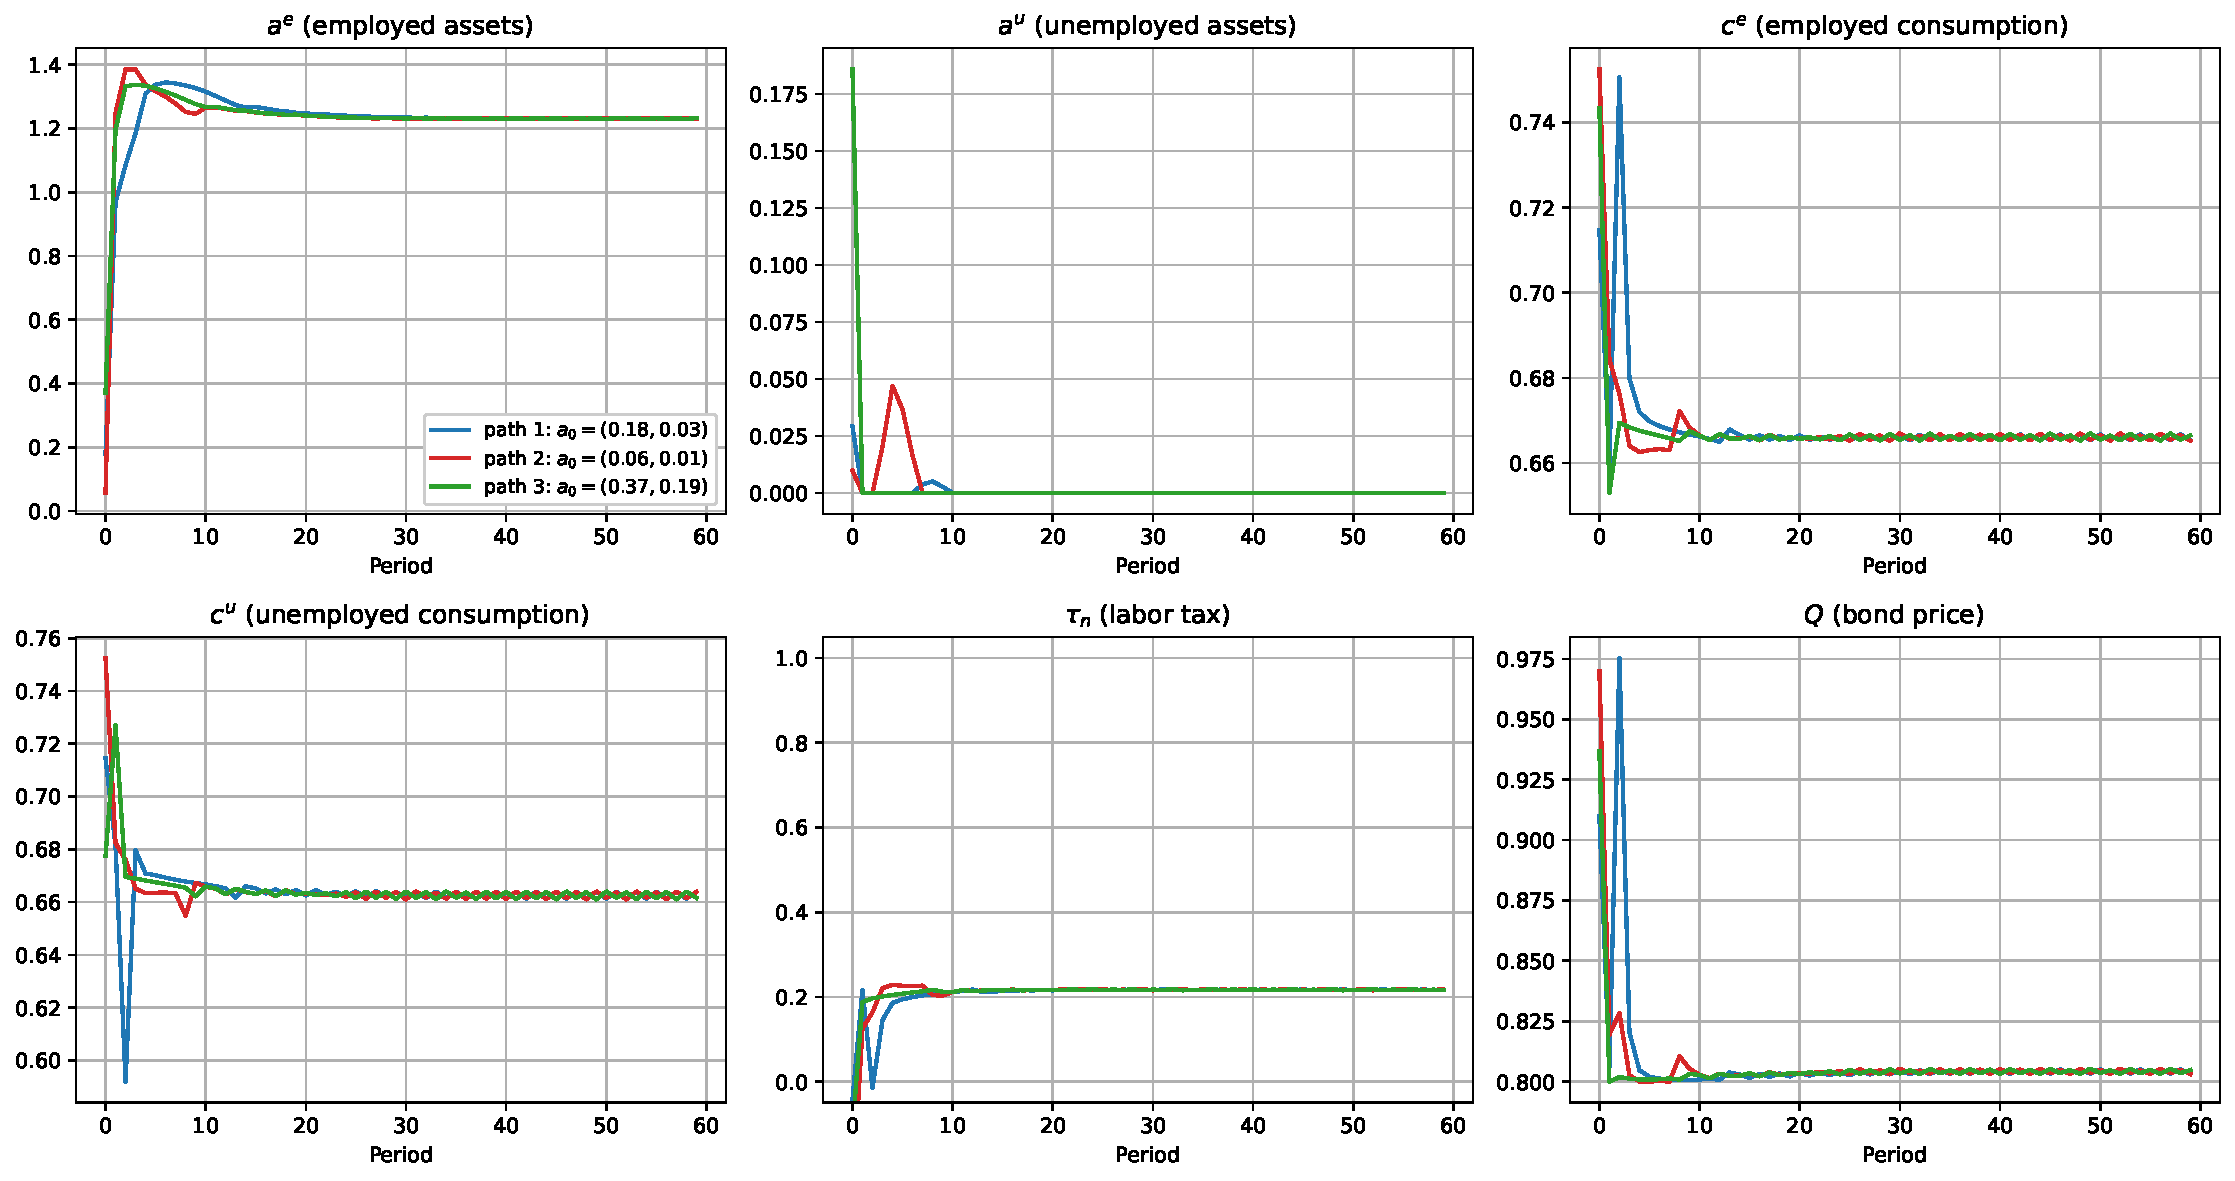
\includegraphics[width=0.92\linewidth]{crra_v6_converge}\\[-0.05cm]
{\tiny A path converging to full self-insurance.}\\[0.12cm]
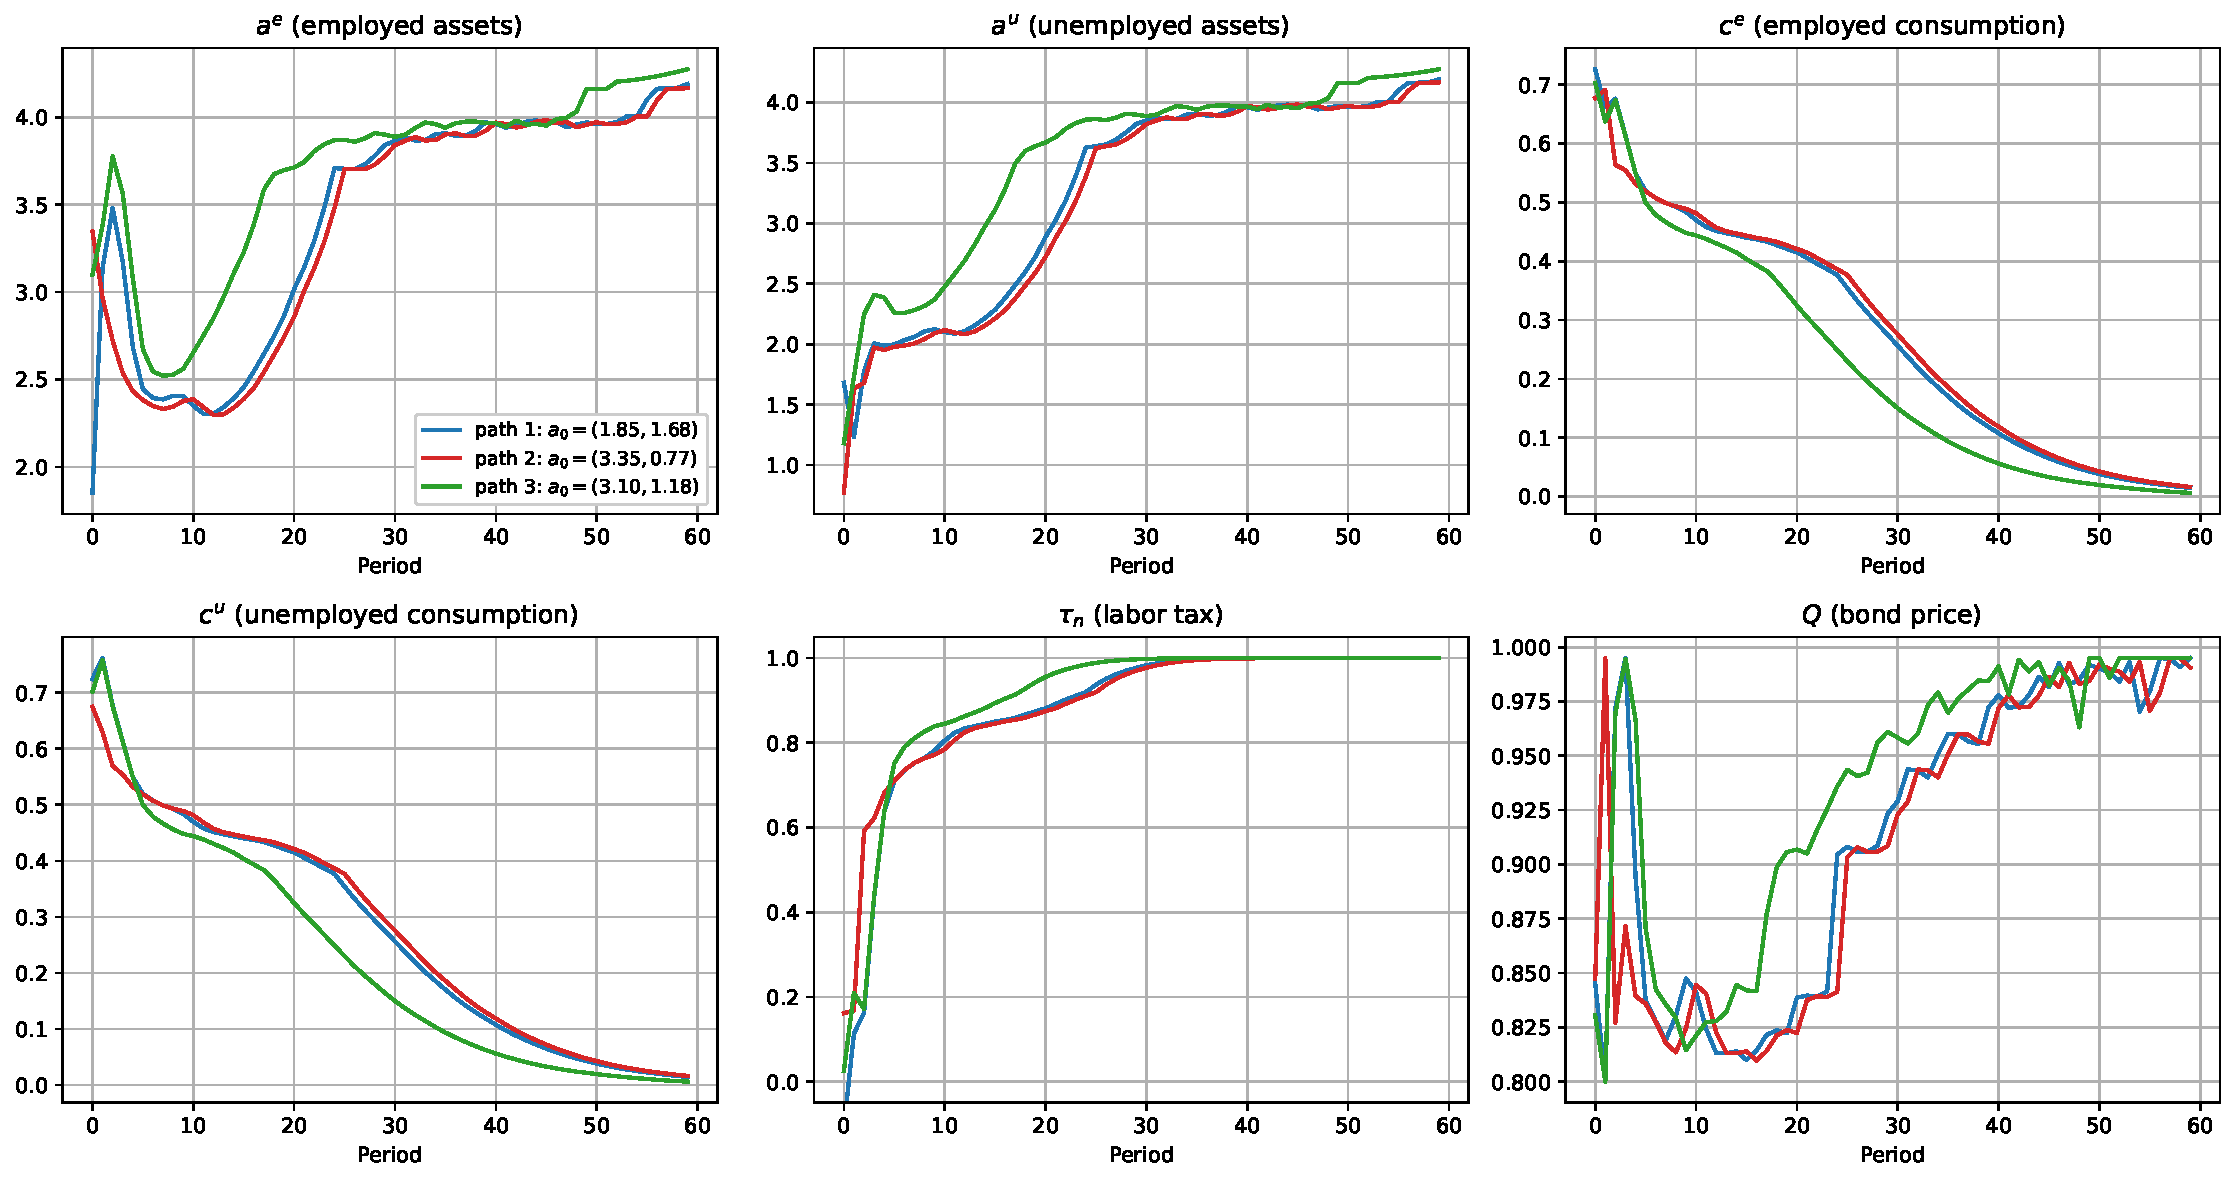
\includegraphics[width=0.92\linewidth]{crra_v6_diverge}\\[-0.05cm]
{\tiny A divergent (immiseration) path from high initial assets. Source: Chien, Feng \& Wen (in progress).}
\end{center}
\end{column}
\end{columns}
\end{frame}

\begin{frame}{The Researcher Becomes a Project Manager}
\textbf{As AI supplies the throughput, your job shifts from \emph{doing every step by hand} (the old artisan mode) to \emph{directing the line}.} Like a plant manager, you own three things:
\smallskip
\begin{itemize}\small
    \item \textbf{Vision} --- a sharp research \emph{goal}: what is the end product, and what makes it \emph{interesting}?
    \item \textbf{Deliverables} --- the intermediate steps and products the goal decomposes into (the milestones).
    \item \textbf{Workflow} --- the \emph{assembly line} from inputs to result: order the stations, and assign each to AI (throughput) or to yourself (judgment).
\end{itemize}
\vspace{-2mm}
\begin{center}
\begin{tikzpicture}[
    every node/.style={font=\scriptsize},
    st/.style={draw, rounded corners=2pt, align=center, minimum height=0.85cm, text width=1.55cm, inner sep=2pt},
    a/.style={-{Stealth[length=1.6mm]}, semithick},
    sub/.style={font=\tiny\itshape, text=black!60},
]
\node[draw, rounded corners=3pt, fill=blue!6, align=center, text width=10.5cm, minimum height=0.62cm] (pm) at (5.25,1.15)
    {\textbf{You, the project manager}\; --- \; set the \textbf{goal} $\cdot$ define the \textbf{deliverables} $\cdot$ design the \textbf{line}};
\node[st, fill=gray!8]    (s1) at (0,0)    {\textbf{Seed}};
\node[st, fill=blue!8]    (s2) at (2.1,0)  {\textbf{Audit}};
\node[st, fill=blue!8]    (s3) at (4.2,0)  {\textbf{Extend on paper}};
\node[st, fill=green!12]  (s4) at (6.3,0)  {\textbf{Prototype}};
\node[st, fill=yellow!18, text width=1.9cm] (s5) at (8.4,0)  {\textbf{Debug $\to$ architecture}};
\node[st, fill=green!16]  (s6) at (10.5,0) {\textbf{Result}};
\node[sub] at (0,-0.66)    {RA solver};
\node[sub] at (2.1,-0.66)  {you check};
\node[sub] at (4.2,-0.66)  {TeX-first};
\node[sub] at (6.3,-0.66)  {AI writes v1};
\node[sub] at (8.4,-0.66)  {failures teach};
\node[sub] at (10.5,-0.66) {bistable long run};
\foreach \i/\j in {s1/s2,s2/s3,s3/s4,s4/s5,s5/s6} \draw[a] (\i) -- (\j);
\draw[a, dashed, black!45] (pm) -- (s2);
\draw[a, dashed, black!45] (pm) -- (s5);
\end{tikzpicture}
\end{center}
\vspace{-2mm}
\begin{takeawaybox}\small
The Case A ladder you just saw \emph{was} this line: audit $\to$ extend on paper $\to$ prototype $\to$ debug-into-architecture $\to$ validate. You never worked the conveyor --- you \textbf{designed} it and stood at the \textbf{judgment gates}.
\end{takeawaybox}
\end{frame}

%=============================================================================
\section{Case B --- GRAM (Context Is the Bottleneck)}

\sectiondivider{Case B --- GRAM}{Capability is not the bottleneck; \emph{context} is}

\begin{frame}{Capability Is Not the Bottleneck --- Context Is}
\textbf{The same frontier tools, available to everyone, produce dramatically different research outcomes --- because of how the human supplies \emph{context}.}
\medskip
\begin{itemize}
    \item Modern models are already capable enough for sophisticated quantitative-macro work\ldots
    \item \ldots but \textbf{ungrounded}, they fail in characteristic ways:
    \begin{itemize}
        \item confident \emph{hallucinated} citations with real-looking DOIs;
        \item plausible-but-wrong methods (valid elsewhere, invalid \emph{here});
        \item knowledge-cutoff blindness (the actual algorithm is post-cutoff);
        \item fluent, unsourced prose you cannot check.
    \end{itemize}
\end{itemize}
\medskip
\begin{cautionbox}\small
The bottleneck is not raw capability --- it is getting the \emph{right field-specific context}, \textbf{with its conditions of validity}, in front of the model.
\end{cautionbox}
\smallskip
{\scriptsize Based on Feng, Miao, Xie, Zhong \& Zhou (2026), \emph{GRAM: Generative Reasoning and Augmented Modeling for Quantitative Macroeconomics} (instructor WIP).}
\end{frame}

\begin{frame}{Four Ways to Give an LLM Context}
\begin{center}
\begin{tikzpicture}[
    every node/.style={font=\scriptsize},
    box/.style={draw, rounded corners=2pt, align=center, minimum height=0.5cm, text width=2.15cm, inner sep=2pt, fill=gray!8},
    gbox/.style={draw=green!45!black, rounded corners=2pt, align=center, minimum height=0.5cm, text width=2.15cm, inner sep=2pt, fill=green!8},
    a/.style={-{Stealth[length=1.5mm]}, semithick},
    outlbl/.style={font=\scriptsize\itshape},
]
\node[box] (h1) at (0,3) {\textbf{Naive LLM}};
\node[box] (h2) at (3,3) {\textbf{In-context stuffing}};
\node[box] (h3) at (6,3) {\textbf{RAG (embedding)}};
\node[gbox] (h4) at (9,3) {\textbf{GRAM (typed graph)}};
\node[box] (p1) at (0,2) {query $\to$ LLM};
\node[box] (p2) at (3,2) {pasted text + query $\to$ LLM};
\node[box] (p3) at (6,2) {top-$k$ passages + query $\to$ LLM};
\node[gbox] (p4) at (9,2) {ranked subgraph + query $\to$ LLM};
\node[box] (a1) at (0,1) {answer};
\node[box] (a2) at (3,1) {answer};
\node[box] (a3) at (6,1) {answer};
\node[gbox] (a4) at (9,1) {\textbf{cited} answer};
\foreach \i in {1,2,3,4} { \draw[a] (h\i) -- (p\i); \draw[a] (p\i) -- (a\i); }
\node[outlbl, red!60!black] at (0,0.35) {silent structural failure};
\node[outlbl] at (3,0.35) {bounded by curation};
\node[outlbl, orange!70!black] at (6,0.35) {surface-similar; structure-blind};
\node[outlbl, green!45!black] at (9,0.35) {ranked + \textbf{condition-aware}};
\end{tikzpicture}
\end{center}
\vspace{-1mm}
\begin{takeawaybox}\small
Only GRAM adds \textbf{condition-aware retrieval}: a method is retrieved \emph{together with the conditions under which it holds}. Fact lookup and compositional retrieval are not enough.
\end{takeawaybox}
\end{frame}

\begin{frame}{Why Naive RAG Falls Short: Economics Is Math \emph{and} Narrative}
\textbf{Two retrieval traditions each handle only \emph{one} side of a paper. Economics papers are \emph{both} math (the analytical scaffold) and prose (the model's anatomy and mechanisms) at once.}
\smallskip
\begin{center}\footnotesize
\renewcommand{\arraystretch}{1.2}
\begin{tabular}{p{3.4cm}p{3.5cm}p{4.4cm}}
\toprule
\textbf{Math info retrieval} & \textbf{Social-science / legal RAG} & \textbf{Economics --- GRAM} \\
\midrule
Pure-math papers & Qualitative prose (e.g.\ LegalGraphRAG) & \emph{Both at once} \\
Unit: theorem / equation & Unit: case / statute / note & Unit: typed economic axes, \emph{equations carried inside} \\
Structure from embedding similarity & Typed graph injects domain knowledge & Typed graph $+$ textbook canon \\
\emph{Strong on math, blind to prose} & \emph{Strong on prose, no math} & \emph{Math is analysis; prose is mechanism} \\
\bottomrule
\end{tabular}
\end{center}
\smallskip
\begin{conceptbox}\small
A flat embedding store indexes \emph{surface text} and respects neither structure. GRAM \textbf{sorts out the structure}: one typed extraction carries both --- the prose anatomy with its math inside --- so retrieval matches the \emph{conditions} a question needs, not just the most-similar passage.
\end{conceptbox}
\end{frame}

\begin{frame}{PromptEcon: A Shared Basis for Models}
\textbf{The engine of Stage 3 --- one fixed basis for the anatomy of \emph{any} structural macro model:}
\smallskip
\begin{center}
\begin{tikzpicture}[
    every node/.style={font=\scriptsize},
    b/.style={draw, rounded corners=2pt, align=center, minimum height=0.95cm, text width=2.55cm, inner sep=2pt},
    a/.style={-{Stealth[length=1.6mm]}, semithick},
]
\node[b, fill=gray!8] (in) at (0,0) {paper\\(Markdown)};
\node[b, fill=blue!8] (def) at (3.1,0) {\textbf{Define} a structure\\{\tiny 3 blocks $\to$ 9 categories\\ $\to$ 51 axes + 7 typed edges}};
\node[b, fill=green!10] (ext) at (6.4,0) {\textbf{Extract} each\\ paper into it\\{\tiny key elements + math}};
\node[b, fill=yellow!18] (con) at (9.7,0) {\textbf{Connect} papers\\{\tiny shared coordinates}};
\foreach \x/\y in {in/def,def/ext,ext/con} \draw[a] (\x) -- (\y);
\node[b, fill=green!14, text width=4.2cm] (back) at (9.7,-1.55) {$=$ condition-aware backbone of the RAG};
\draw[a] (con) -- (back);
\end{tikzpicture}
\end{center}
\smallskip
\begin{conceptbox}\small
\textbf{The 51 axes are the unit of retrieval.} Because every paper is projected onto the \emph{same} coordinates, papers align by typed concept --- and a query can demand the axis (e.g.\ \texttt{solution\_method}) that fits its stated conditions.
\end{conceptbox}
\end{frame}

\begin{frame}{Payoff --- and Where This Goes}
\begin{itemize}
    \item \textbf{Replicate in days:} an empirical researcher opened an \emph{unfamiliar} codebase, paired it with an agent, and in days replicated the model and solved computational problems the original author had been stuck on.
    \item \textbf{$\sim$10$\times$ throughput:} a computational researcher reached a roughly ten-fold improvement on \emph{their own} code with an AI assistant in the loop.
\end{itemize}
\medskip
\begin{takeawaybox}\small
\textbf{Forward pointers:} the retrieval mechanics (embeddings, RAG, GraphRAG) $\to$ Lec.\ 8; agentic orchestration of multi-step research $\to$ Lec.\ 9. Building such infrastructure is \textbf{Capstone Track D}.
\end{takeawaybox}
\end{frame}

%=============================================================================
\section{AI-for-Research Map \& the Causation Guardrail}

\sectiondivider{AI-for-Research Map \& the Causation Guardrail}{Where AI helps across the research pipeline --- and the one claim it must never make for you}

\begin{frame}{AI Tools for Economic Research: A Map}
\begin{center}
\renewcommand{\arraystretch}{1.3}
\begin{tabular}{|l|l|l|}
\hline
\textbf{Task} & \textbf{AI Approach} & \textbf{Economic Application} \\
\hline
Prediction & Supervised learning & Forecasting, scoring, targeting \\
Pattern discovery & Unsupervised learning & Consumer types, factor models \\
Text analysis & NLP / LLMs & FOMC, speeches, filings \\
Causal inference & ML + IV / DiD & Heterogeneous treatment effects \\
Structural estimation & RL / DL & Solving complex macro models \\
Literature review & RAG + LLM & Systematic reviews, survey papers \\
Coding & Agentic AI & Data cleaning, estimation, tables \\
\hline
\end{tabular}
\end{center}

\vfill
\begin{flushright}\footnotesize
\textit{The rows above are the material covered in}\\[1pt]\bookAIforEcon
\end{flushright}
\end{frame}

\begin{frame}{AI in Economic Research: Concrete Examples (I)}
\begin{itemize}\small
\item \textbf{Prediction (supervised).} Nowcast GDP / inflation from high-frequency and alternative data (card spending, satellite night-lights); predict firm default or earnings surprises from filings. \hfill{\scriptsize(Lec.\ 3)}
\medskip
\item \textbf{Pattern discovery (unsupervised).} Topic models / embeddings on FOMC minutes and earnings calls to surface latent themes; cluster firms or households into types from panel data. \hfill{\scriptsize(Lec.\ 7)}
\medskip
\item \textbf{Text as data (NLP / LLMs).} Score hawkish/dovish tone in central-bank language; extract firm-level risk exposure from 10-K Item~1A; build a policy-uncertainty index from newspapers (Baker--Bloom--Davis). \hfill{\scriptsize(Lec.\ 7--8)}
\end{itemize}
\vfill
{\footnotesize\textit{The map's first rows, made concrete: AI turns messy inputs into \textbf{measures} and \textbf{datasets}.}}
\end{frame}

\begin{frame}{AI in Economic Research: Concrete Examples (II)}
\begin{itemize}\small
\item \textbf{Causal inference (ML $+$ IV/DiD).} Double/debiased ML to control high-dimensional confounders (returns to schooling); causal forests for heterogeneous treatment effects (who gains from a policy); synthetic control for a single treated unit (Abadie). \hfill{\scriptsize(Lec.\ 3)}
\medskip
\item \textbf{Structural estimation (DL / RL).} Neural-network solutions of high-dimensional dynamic models (Aiyagari, Krusell--Smith); deep learning for the Bellman / Euler equations where grids break down. \hfill{\scriptsize(Lec.\ 4--6; \textbf{Capstone A})}
\medskip
\item \textbf{Literature \& coding (RAG $+$ agentic).} GraphRAG over NBER/arXiv for systematic surveys (the T1.2 GRAM case); an agent builds the data\,$\to$\,clean\,$\to$\,estimate\,$\to$\,table pipeline and replicates a paper from public data. \hfill{\scriptsize(Lec.\ 8--10; \textbf{Capstone C, D})}
\end{itemize}
\vfill
\begin{cautionbox}\footnotesize
\textbf{The guardrail.} AI supplies the \emph{prediction, measurement, and computation}. Identification --- \emph{why} a number is causal --- remains the economist's job: prediction $\neq$ causation.
\end{cautionbox}
\end{frame}

\begin{frame}{AI Strengths and Limitations for Economists}
\begin{columns}[T]
    \column{0.48\textwidth}
    \begin{tcolorbox}[colback=green!5, colframe=green!40!black, title=Where AI Excels]
    \begin{itemize}
        \item High-dimensional pattern recognition
        \item Text analysis at scale (FOMC, patents, filings)
        \item Constructing new datasets from unstructured data
        \item Automating repetitive coding and cleaning tasks
        \item Solving high-dimensional optimization problems (DL for macro models)
    \end{itemize}
    \end{tcolorbox}

    \column{0.48\textwidth}
    \begin{tcolorbox}[colback=red!5, colframe=red!40!black, title=Where Economists Add Value]
    \begin{itemize}
        \item Identification and causal reasoning
        \item Economic structure: what are the right state variables?
        \item Welfare analysis and normative judgment
        \item Designing the question AI answers
        \item Validating model outputs against economic theory
    \end{itemize}
    \end{tcolorbox}
\end{columns}

\medskip
\begin{center}
\footnotesize\textit{``AI compensates for human cognitive limitations in pattern matching but lacks the human capacity for causal explanation.'' --- Sargent (2023). Lec.\ 7 T3b catalogues LLM limitations; Lec.\ 9 T5 turns them into a publication-grade audit checklist.}
\end{center}
\end{frame}

%=============================================================================
\section{A Live Measurement Example (instructor WIP)}

\sectiondivider{A Live Measurement Example}{Instructor work-in-progress: measuring what AI can attempt vs.\ finish}

\begin{frame}{Measuring AI as Cognitive Capital: From the Capability Index to Data}
\begin{itemize}
\item \textbf{Bridge.} The task-level CES slide (T1.1) carried two unobservables: an AI-capability index $\theta_i$ and an adoption margin $E_i$. \emph{Can we measure them?} Merge the \textbf{Anthropic Economic Index} (observed Claude usage) onto \textbf{O\*NET} tasks.
\item \textbf{Per occupation:} sort tasks \emph{most-important-first}, then trace cumulative AI-usage share against cumulative task-importance weight $\Rightarrow$ a Lorenz-style deployment curve.
\end{itemize}
\vspace{-1mm}
\begin{columns}[T]
    \column{0.40\textwidth}
    \begin{conceptbox}
    \footnotesize
    \textbf{Three deployment indices:}
    \begin{itemize}
        \item \textbf{Signed Gini $G$}: $>0$ = AI on core/important tasks; $<0$ = peripheral.
        \item $|G|$: \emph{sharpness} of the human--AI task split (direction-free).
        \item $\bar{E}$: importance-weighted usage \emph{intensity}.
    \end{itemize}
    \end{conceptbox}
    \column{0.58\textwidth}
    \begin{center}
    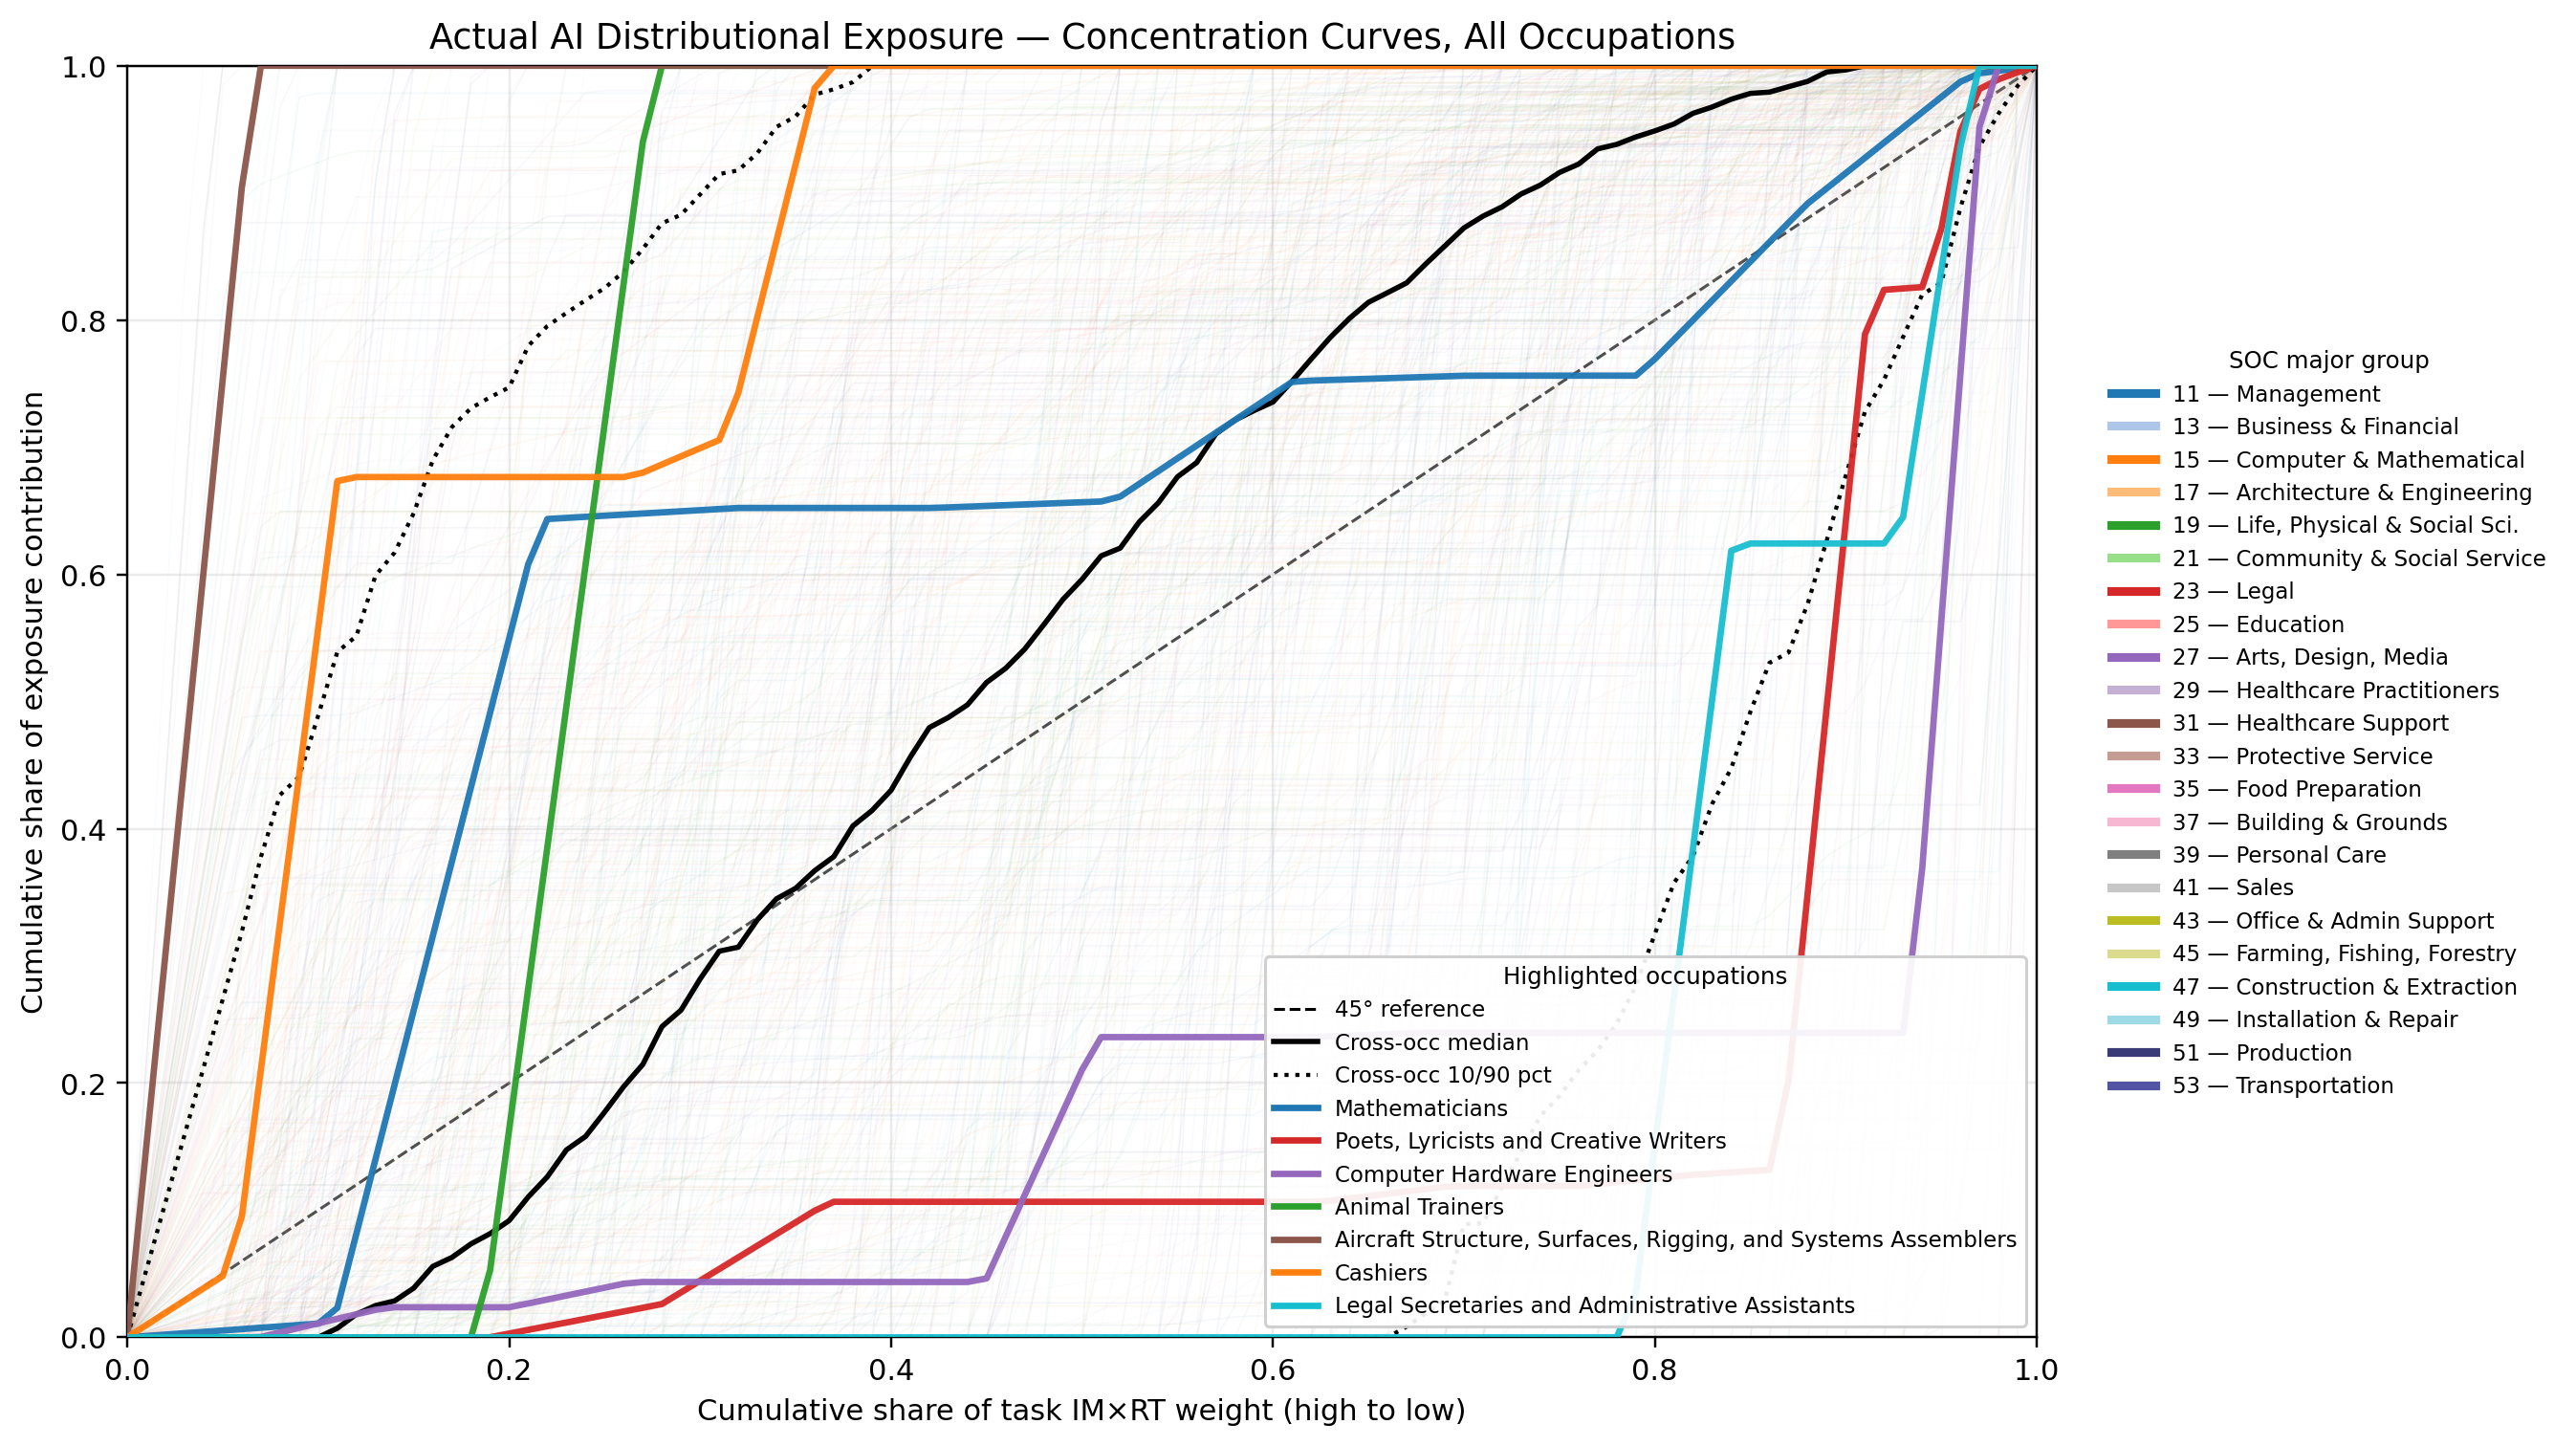
\includegraphics[width=\linewidth,totalheight=4.6cm,keepaspectratio]{figures/spaghetti_distributional_exposure_actual.png}
    \end{center}
\end{columns}
\vspace{-1mm}
\begin{takeawaybox}
\footnotesize
\textbf{Punchline:} AI is a \emph{task-level, unevenly deployed} capability --- the median curve sits well above the 45$^\circ$ line, so usage concentrates on a subset of tasks.
\end{takeawaybox}
\vspace{-1mm}
{\tiny\textit{Usage $=$ observed AEI Claude-conversation share (Mar 2025 vintage), not productivity. Ongoing WIP by the instructor; associations only.}}
\end{frame}

\begin{frame}{Is AI Actually Capable Yet? A Task-Level Capability Index}
\begin{itemize}
\item An LLM rates \emph{every} O\*NET task on two axes (blinded, averaged over 3 passes):
\begin{itemize}
    \item $\mathrm{CAP}_{\text{tech}}$ --- technical coverage: can current AI \emph{attempt} the task? (mean $\sim 0.46$)
    \item $\mathrm{CAP}_{\text{auto}}$ --- autonomous coverage: can it \emph{finish} without human review? (mean $\sim 0.21$)
\end{itemize}
\end{itemize}
\begin{center}
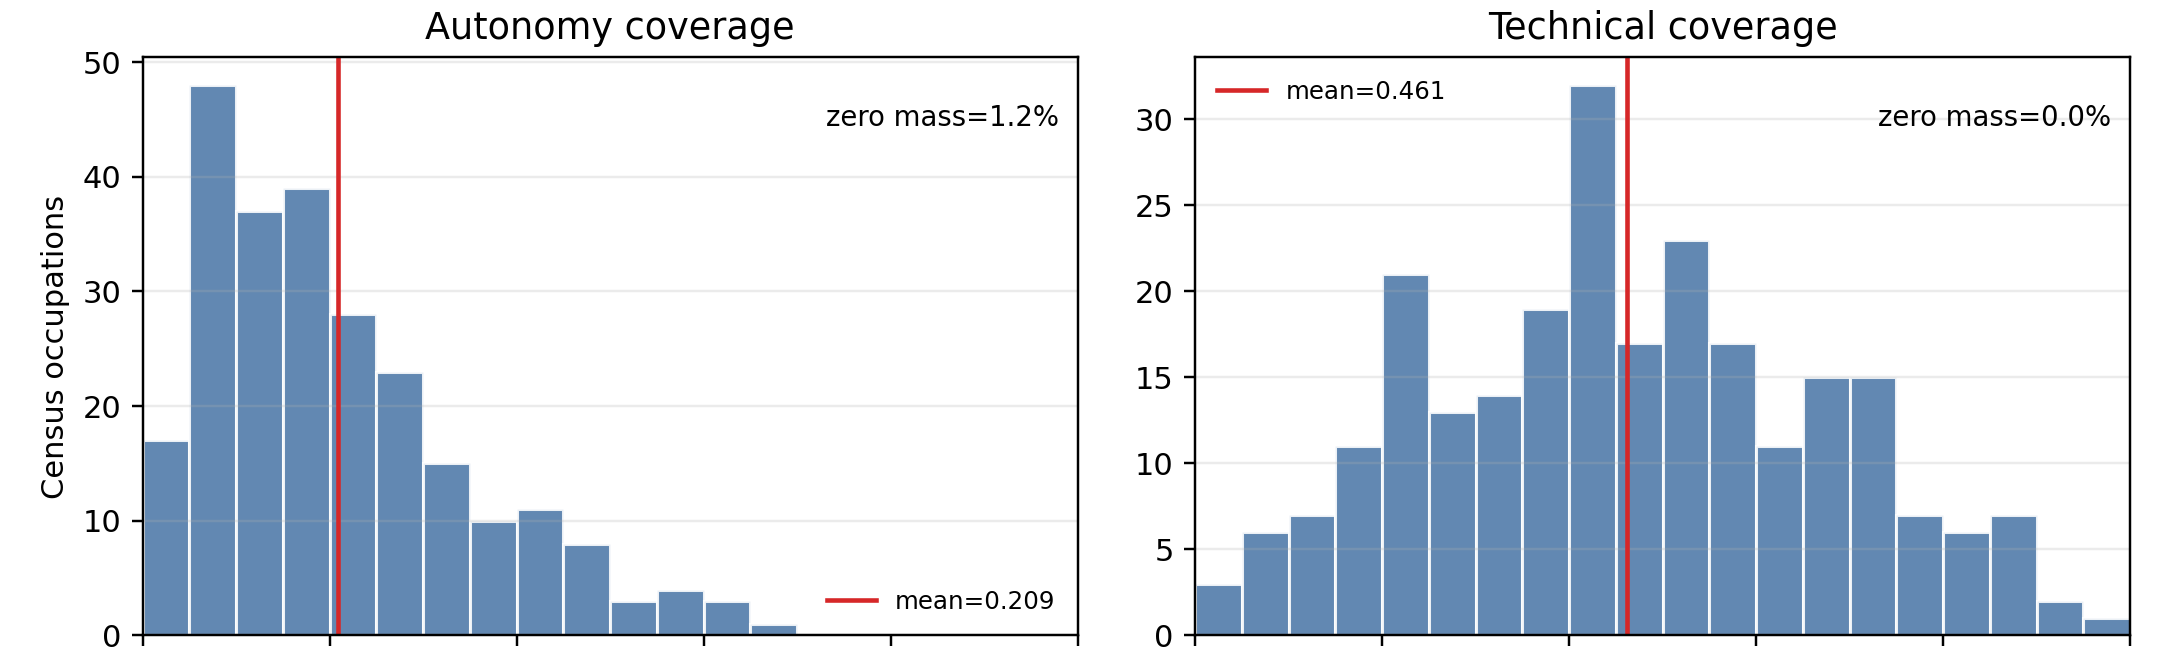
\includegraphics[width=10.5cm,totalheight=4.0cm,keepaspectratio]{figures/capability_index_toprow.png}
\end{center}
\vspace{-1mm}
\begin{takeawaybox}
\footnotesize
\textbf{AI can \emph{attempt} much but \emph{finish} unsupervised little} --- consistent with Acemoglu's ``$\sim$4.6\% of tasks exposed.''
\end{takeawaybox}
\vspace{-1mm}
\begin{cautionbox}
\footnotesize
\textbf{Caveat:} this is an LLM \emph{self-rating} (blinded, 3-pass averaged) --- a model judgment, not external ground truth.
\end{cautionbox}
\end{frame}

%=============================================================================
% House-style bridge closer (matches Lec05/Lec09): restate the act, hand off.
\begin{frame}{Bridge: The Proof Is In --- Now Make It Your Practice}
\textbf{Act 1.2 delivered the evidence. AI co-developed a dynamic model (DeepRamsey); context --- not capability --- emerged as the binding constraint (GRAM); and the task-level index showed AI can \emph{attempt} much but \emph{finish} unsupervised little.}

\vspace{0.25cm}
\begin{itemize}
  \item You have seen two live cases and one measurement project --- with causation as the standing guardrail: AI drafts, computes, and searches; \emph{you} own identification and the causal claim.
  \item \textbf{Next (1.3):} how this course works --- the two-arc roadmap, the research-architect stance and tooling, and the replication-first capstone.
\end{itemize}

\vspace{0.3cm}
\begin{center}
\footnotesize\textit{Arc: 1.1 FRAME (cognitive capital) $\;\to\;$ \textbf{1.2 PROOF} (AI doing research) $\;\to\;$ 1.3 PRACTICE (course $+$ capstone).}
\end{center}
\end{frame}

\end{document}
